\documentclass{article}\usepackage[]{graphicx}\usepackage[]{color}
% maxwidth is the original width if it is less than linewidth
% otherwise use linewidth (to make sure the graphics do not exceed the margin)
\makeatletter
\def\maxwidth{ %
  \ifdim\Gin@nat@width>\linewidth
    \linewidth
  \else
    \Gin@nat@width
  \fi
}
\makeatother

\definecolor{fgcolor}{rgb}{0.345, 0.345, 0.345}
\newcommand{\hlnum}[1]{\textcolor[rgb]{0.686,0.059,0.569}{#1}}%
\newcommand{\hlstr}[1]{\textcolor[rgb]{0.192,0.494,0.8}{#1}}%
\newcommand{\hlcom}[1]{\textcolor[rgb]{0.678,0.584,0.686}{\textit{#1}}}%
\newcommand{\hlopt}[1]{\textcolor[rgb]{0,0,0}{#1}}%
\newcommand{\hlstd}[1]{\textcolor[rgb]{0.345,0.345,0.345}{#1}}%
\newcommand{\hlkwa}[1]{\textcolor[rgb]{0.161,0.373,0.58}{\textbf{#1}}}%
\newcommand{\hlkwb}[1]{\textcolor[rgb]{0.69,0.353,0.396}{#1}}%
\newcommand{\hlkwc}[1]{\textcolor[rgb]{0.333,0.667,0.333}{#1}}%
\newcommand{\hlkwd}[1]{\textcolor[rgb]{0.737,0.353,0.396}{\textbf{#1}}}%
\let\hlipl\hlkwb

\usepackage{framed}
\makeatletter
\newenvironment{kframe}{%
 \def\at@end@of@kframe{}%
 \ifinner\ifhmode%
  \def\at@end@of@kframe{\end{minipage}}%
  \begin{minipage}{\columnwidth}%
 \fi\fi%
 \def\FrameCommand##1{\hskip\@totalleftmargin \hskip-\fboxsep
 \colorbox{shadecolor}{##1}\hskip-\fboxsep
     % There is no \\@totalrightmargin, so:
     \hskip-\linewidth \hskip-\@totalleftmargin \hskip\columnwidth}%
 \MakeFramed {\advance\hsize-\width
   \@totalleftmargin\z@ \linewidth\hsize
   \@setminipage}}%
 {\par\unskip\endMakeFramed%
 \at@end@of@kframe}
\makeatother

\definecolor{shadecolor}{rgb}{.97, .97, .97}
\definecolor{messagecolor}{rgb}{0, 0, 0}
\definecolor{warningcolor}{rgb}{1, 0, 1}
\definecolor{errorcolor}{rgb}{1, 0, 0}
\newenvironment{knitrout}{}{} % an empty environment to be redefined in TeX

\usepackage{alltt}
\usepackage[]{graphicx}
\usepackage[]{color}
\usepackage[colorlinks=true,linkcolor=blue]{hyperref}
% maxwidth is the original width if it is less than linewidth
% otherwise use linewidth (to make sure the graphics do not exceed the margin)


\makeatletter
\def\maxwidth{ %
  \ifdim\Gin@nat@width>\linewidth
    \linewidth
  \else
    \Gin@nat@width
  \fi
}
\makeatother

\definecolor{fgcolor}{rgb}{0.345, 0.345, 0.345}
%\newcommand{\hlnum}[1]{\textcolor[rgb]{0.686,0.059,0.569}{#1}}%
%\newcommand{\hlstr}[1]{\textcolor[rgb]{0.192,0.494,0.8}{#1}}%
%\newcommand{\hlcom}[1]{\textcolor[rgb]{0.678,0.584,0.686}{\textit{#1}}}%
%\newcommand{\hlopt}[1]{\textcolor[rgb]{0,0,0}{#1}}%
%\newcommand{\hlstd}[1]{\textcolor[rgb]{0.345,0.345,0.345}{#1}}% 
%\newcommand{\hlkwa}[1]{\textcolor[rgb]{0.161,0.373,0.58}{\textbf{#1}}}%
%\newcommand{\hlkwb}[1]{\textcolor[rgb]{0.69,0.353,0.396}{#1}}%
%\newcommand{\hlkwc}[1]{\textcolor[rgb]{0.333,0.667,0.333}{#1}}%
%\newcommand{\hlkwd}[1]{\textcolor[rgb]{0.737,0.353,0.396}{\textbf{#1}}}%
%\let\hlipl\hlkwb

\usepackage{framed}
\makeatletter

%\newenvironment{kframe}{%
% \def\at@end@of@kframe{}%
% \ifinner\ifhmode%
%  \def\at@end@of@kframe{\end{minipage}}%
%  \begin{minipage}{\columnwidth}%
% \fi\fi%
% \def\FrameCommand##1{\hskip\@totalleftmargin \hskip-\fboxsep
% \colorbox{shadecolor}{##1}\hskip-\fboxsep
     % There is no \\@totalrightmargin, so:
%     \hskip-\linewidth \hskip-\@totalleftmargin \hskip\columnwidth}%
% \MakeFramed {\advance\hsize-\width
%   \@totalleftmargin\z@ \linewidth\hsize
%   \@setminipage}}%
% {\par\unskip\endMakeFramed%
% \at@end@of@kframe}
%\makeatother

\definecolor{shadecolor}{rgb}{.97, .97, .97}
\definecolor{messagecolor}{rgb}{0, 0, 0}
\definecolor{warningcolor}{rgb}{1, 0, 1}
\definecolor{errorcolor}{rgb}{1, 0, 0}
%\newenvironment{knitrout}{}{} % an empty environment to be redefined in TeX

\usepackage{alltt}
\usepackage{listings}

\definecolor{mygreen}{rgb}{0,0.6,0}
\definecolor{mygray}{rgb}{0.5,0.5,0.5}
\definecolor{mymauve}{rgb}{0.58,0,0.82}

\lstset{ 
  backgroundcolor=\color{white},   % choose the background color; you must add \usepackage{color} or \usepackage{xcolor}; should come as last argument
  basicstyle=\footnotesize,        % the size of the fonts that are used for the code
  breakatwhitespace=false,         % sets if automatic breaks should only happen at whitespace
  breaklines=true,                 % sets automatic line breaking
  captionpos=,                    % sets the caption-position to bottom
  commentstyle=\color{mygreen},    % comment style
  deletekeywords={...},            % if you want to delete keywords from the given language
  escapeinside={\%*}{*)},          % if you want to add LaTeX within your code
  extendedchars=true,              % lets you use non-ASCII characters; for 8-bits encodings only, does not work with UTF-8
  firstnumber=1,                % start line enumeration with line 1000
  frame=single,	                   % adds a frame around the code
  keepspaces=true,                 % keeps spaces in text, useful for keeping indentation of code (possibly needs columns=flexible)
  keywordstyle=\color{blue},       % keyword style
  language=Python,                 % the language of the code
  morekeywords={*,...},            % if you want to add more keywords to the set
  numbers=left,                    % where to put the line-numbers; possible values are (none, left, right)
  numbersep=5pt,                   % how far the line-numbers are from the code
  numberstyle=\tiny\color{mygray}, % the style that is used for the line-numbers
  rulecolor=\color{black},         % if not set, the frame-color may be changed on line-breaks within not-black text (e.g. comments (green here))
  showspaces=false,                % show spaces everywhere adding particular underscores; it overrides 'showstringspaces'
  showstringspaces=false,          % underline spaces within strings only
  showtabs=false,                  % show tabs within strings adding particular underscores
  stepnumber=1,                    % the step between two line-numbers. If it's 1, each line will be numbered
  stringstyle=\color{mymauve},     % string literal style
  tabsize=2,	                   % sets default tabsize to 2 spaces
  title=\lstname                   % show the filename of files included with \lstinputlisting; also try caption instead of title
}
\IfFileExists{upquote.sty}{\usepackage{upquote}}{}
\begin{document}

\section{Introduction}

\subsection{How is particulate matter analyzed?}

The PM sensor has several components to measure the particles in the air -- remember, we don't know what the make up of these particles might be -- but we can get an estimate of their size distribution. We have written the code to collect particles smaller than 1$\mu$m, 2.5$\mu$m and 10$\mu$m. 

Figure~\ref{fig:hpsensor} is a schematic of the particle sensor made by Honeywell (HPM Series --- Particulate Matter Sensors 32322550HP). The one we are using is made by Plantower. As a Chinese company, most of their literature is in Chinese, so I didn't find something that I could interpret for us. 

\begin{figure}
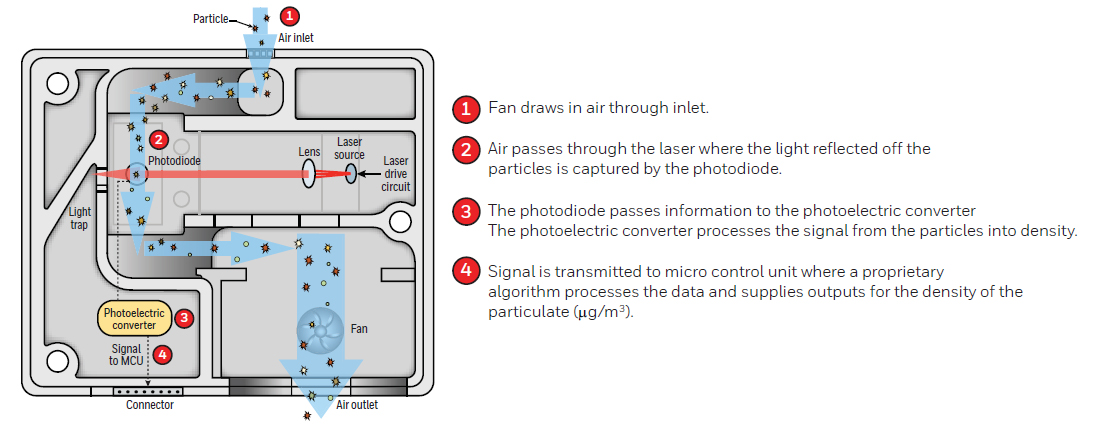
\includegraphics[width=1.00\textwidth]{images/4_SensorSchematic}
\caption{Schematic of Honeywell Particulate Matter Sensor. A laser light source illuminates a particle as it is pulled through the detection chamber. As particles pass through the laser beam, the light reflects off the particles and is recorded on the photo or light detector. The light is then analyzed and converted to an electrical signal to calculate particle concentration.}
\label{fig:hpsensor}
\end{figure}

Our sensors can generate several categories of PM data. Using a laser and light defraction, the number and size of the particles can be estimated (Figure~\ref{fig:defraction}).

\begin{figure}
\includegraphics[width=0.70\textwidth]{images/4_Measurement-principle}
\caption{In particle size measurements using light scattering (DLS), a laser beam is scattered on very small, finely dispersed particles in a highly diluted matrix. 
The scattered light of each particle will then interfere with each other. Since the particles constantly change locations, the position of the scattering centers changes with respect to each other and the interferences lead to small fluctuations in scattering intensity (this explains the name ``dynamic'' light scattering).}
\label{fig:defraction}
\end{figure}

\section{Data Collection}
\subsection{What data is collected by the PMS5003?}

The PMS5003 generates the following data: 

\begin{description}
  \item[Data 1] refers to PM1.0 concentration unit $\mu$g/m$^3$(CF=1,standard particle)\footnote{The Asterisk on Data 1 and Data 4 is defined on the same page as ``Note: CF=1 should be used in the factory environment''}
  \item[Data 2] refers to PM2.5 concentration unit $\mu$g/m$^3$(CF=1,standard particle)
  \item[Data 3] refers to PM10 concentration unit $\mu$g/m$^3$(CF=1,standard particle)
  \item[Data 4] refers to PM1.0 concentration unit $\mu$g/m$^3$(under atmospheric environment)
  \item[Data 5] refers to PM2.5 concentration unit $\mu$g/m$^3$(under atmospheric environment)
  \item[Data 6] refers to concentration unit (under atmospheric environment) $\mu$g/m$^3$
  \item[Data 7] indicates the number of particles with diameter beyond 0.3 $\mu$m in 0.1 L of air.
  \item[Data 8] indicates the number of particles with diameter beyond 0.5 $\mu$m in 0.1 L of air.
  \item[Data 9] indicates the number of particles with diameter beyond 1.0 $\mu$m in 0.1 L of air.
  \item[Data 10] indicates the number of particles with diameter beyond 2.5 $\mu$m in 0.1 L of air.
  \item[Data 11] indicates the number of particles with diameter beyond 5.0 $\mu$m in 0.1 L of air.
  \item[Data 12] indicates the number of particles with diameter beyond 10 $\mu$m in 0.1 L of air

\end{description}

The first set are labeled ``standard'', while the second set are labeled ``atmospheric environment''. What do these measure and how do the ``standard'' ones differ from the ``atmospheric environment'' ones?

It has to do with the density of the air used for calculations. "Standard" refers to the concentration ``corrected'' to the ``standard atmosphere'' which in the US is DEFINED as ``having a temperature of 288.15 K at the sea level 0 km geo-potential height and 1013.25 hPa''. NOTE: 288.15 K equals 25 C and Pa are ``pascals'' which is a meausure of pressure. 

On the other hand, the ``ambient conditions'' are just as the air is ``now'' (whatever temperature and pressure there is). Now what does that mean\ldots

Air being a gas, it is compressible which means that it changes its volume when the pressure changes so when you report concentrations as mass per volume of air it is relevant at what pressure that volume is calculated. For example, if you have a bunch of particles rising in the air in a bubble (no loss of particles, no addition, they're just riding a bubble up in the air) then, as they rise, the pressure drops so what was 1cc at the ground it is now 2cc so the concentration of what was in the bubble is now half without anything actually changing other than the ambient pressure. So, it is common to report concentrations (of anything) as ``x mg per standard m3'' and because we scientist don't like to write much (current example excluded) you'll usually see the ``standard'' being dropped because it is ``implicit''.

For gases it is also common to report concentrations as ``parts per million'' or ``ppm'' and that metric is independent of the volume of air as it represents the number of molecules of the gas in a million molecules of air (including the target gas).

In conclusion, I use the ``standard'' readings for reporting but keep the ``ambient conditions'' for analysis. I haven't used these things in high altitudes so for all my deployments the standard and ambient are very similar. I have written code to extract the standard values only -- but you can certain add the ambient if you want to see if there is a difference -- could be important if you are above 1000 ft in elevation.

\section{Collecting the data}

\subsection{Extract Data From Pi}

    Once the data have been collected, you can extract from the Pi -- Unfortunately, there are several ways to do this and one of them are easier using the VNC interface.
    
\subsubsection{Using RealVNC to transfer data files}

\begin{enumerate}

\item Use RealVNC and VNC into the Raspberry Pi using the Pi's IP adress in the RealVNC search toolbar.

\item Controlling the Raspberry Pi, right click on the VNCServer icon in the toolbar in the upper left near the clock.
\begin{figure}[h]
\centering
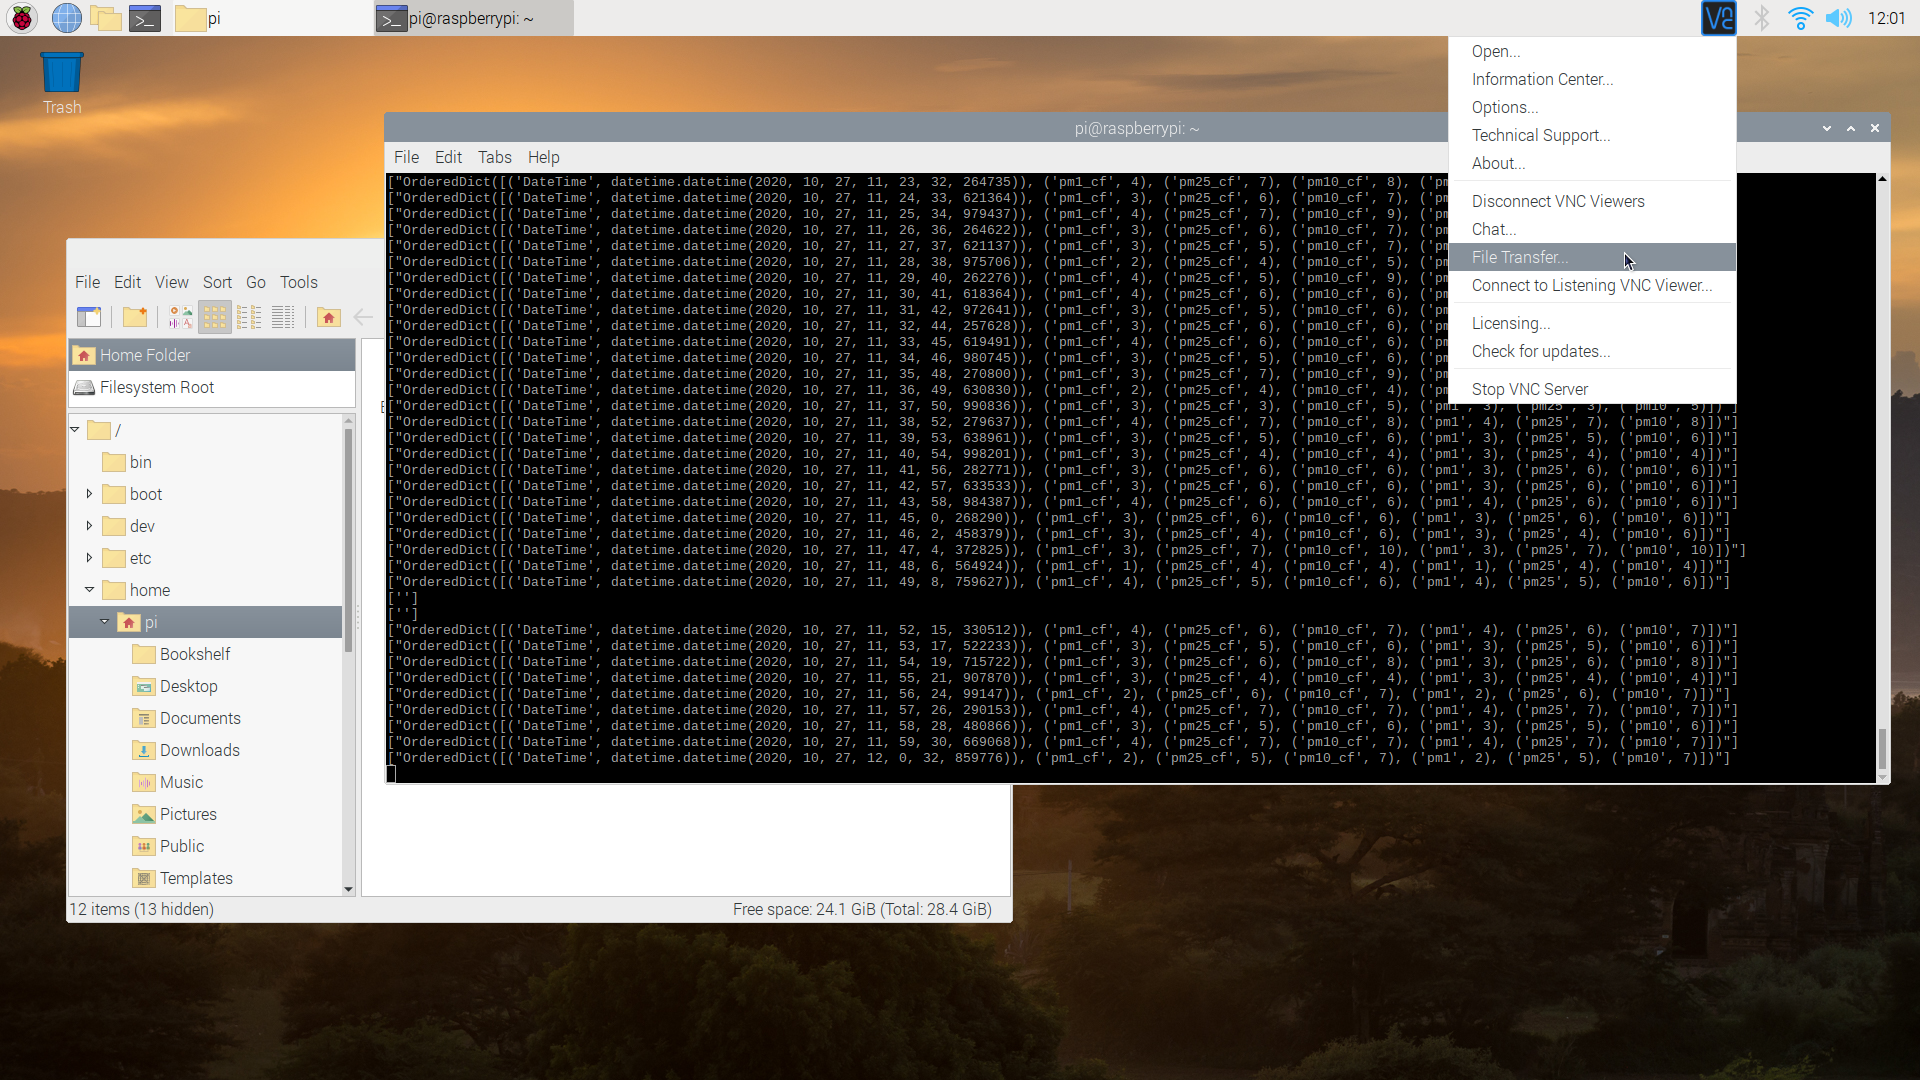
\includegraphics[width=1\textwidth]{images/4_vncserver_ft}
\caption{}
\label{fig:vncserverfiletransfer}
\end{figure}

\item Select \textbf{``File Transfer...''}

\item In the ``File Transfer'' popup window, select \textbf{``Send Files''} in the lower left.
\begin{figure}[h]
\centering
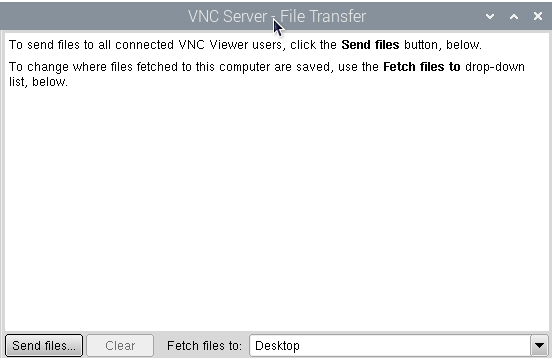
\includegraphics[width=0.80\textwidth]{images/4_vncserver_ft2}
\caption{}
\label{fig:vncserverfiletransfer2}
\end{figure}

\item Then navigate to the file you want to send in the ``Send Files'' popup and click \textbf{``OK''}.
\begin{figure}[h!]
\centering
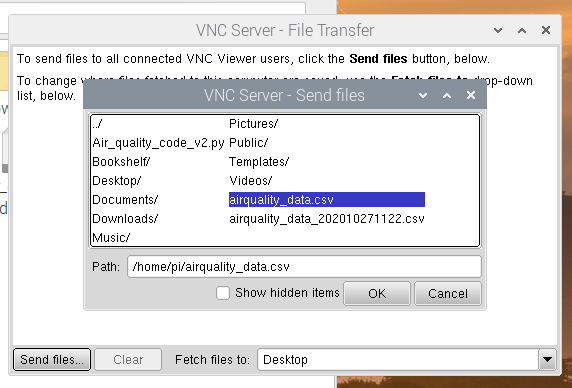
\includegraphics[width=0.80\textwidth]{images/4_vncserver_sf}
\caption{}
\label{fig:vncserversendfiles}
\end{figure}

\item There should be another popup, on your main computer, that will show download manager with your file in it. By default, RealVNC transfers files to your desktop.
\begin{figure}[h!]
\centering
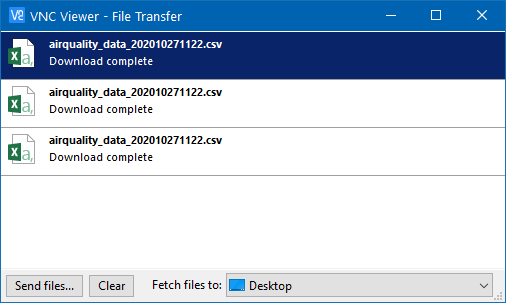
\includegraphics[width=0.80\textwidth]{images/4_vncserver_sfdm}

\label{fig:vncserverdownloadmanager}
\end{figure}

\end{enumerate}

\subsubsection{Alternative Methods For PCs} 

Alternatively, there serveral other alternatives. For example, this \href{https://www.makeuseof.com/tag/copy-data-raspberry-pi-pc/}{webpage describes the issues and 5 not great options} to get data. 

After several attempts to create a cloud folder that you could upload, I found it was far to slow and unreliable. Thus, I recommend using Putty and the following line commands:

\begin{lstlisting}
psftp> open Pi@XXX.XXX.XXX.XXX
\end{lstlisting}

and you will be prompted to enter the password. Once you are in, you can see your files by entering

\begin{lstlisting}
psftp>ls *.csv
\end{lstlisting}


\noindent where all your csv files should be shown. 

Then you'll need to change your local drive (the default one is write protected, creating a signficant obstacle. So, use 

\begin{lstlisting}
psftp>lpwd
\end{lstlisting}
 

\noindent to see your default directly. We are doing to use the download directory and we can change the directory using:

\begin{lstlisting}
psftp>lcd c:/Downloads
\end{lstlisting}

Then we will get the files...

\begin{lstlisting}
psftp>get airquality_data.csv
\end{lstlisting}


and it will be transfered to your local computer... !  Yay!  It only took me 5 hours to figure out and hopefully for you less than 5 min. 

\subsubsection{FOR Macs}

I can't find an easy solution for MACs, use the file transfer function in RealVNC.

\subsection{Processing the data}

We create a script to process the data and allow you to create a reasonably user-friendly dataframe to analyze the data.

\subsection{Remove Double Quotes in CSV}

However, before running the code below, we need to remove all the double quotes, which get in the way of how ``csv'' files are read.

Opened the document up in Rstdudio. Use the edit menu and select "search and replace". Search for double quotes (") and leave the place for ``Replace'' blank, i.e. don't enter anythning. Then replace all. Then you can read the csv into R. 

\begin{knitrout}
\definecolor{shadecolor}{rgb}{0.969, 0.969, 0.969}\color{fgcolor}\begin{kframe}
\begin{alltt}
\hlstd{filepath.csv} \hlkwb{=} \hlstr{"/home/CAMPUS/mwl04747/github/EJnPi/data/Air_Quality.csv"}
\hlstd{filepath.csv} \hlkwb{=} \hlstr{"/home/CAMPUS/mwl04747/github/EJnPi/data/Complete_airquality_data2.csv"}
\hlstd{filepath.csv} \hlkwb{=} \hlstr{"/home/CAMPUS/mwl04747/github/EJnPi/data/201104_Complete_airquality.csv"}
\hlstd{rawdata} \hlkwb{=} \hlkwd{read.csv}\hlstd{(filepath.csv)}

\hlkwd{names}\hlstd{(rawdata)}\hlkwb{=} \hlkwd{c}\hlstd{(}\hlstr{"X1"}\hlstd{,} \hlstr{"X2"}\hlstd{,} \hlstr{"Month"}\hlstd{,} \hlstr{"Day"}\hlstd{,} \hlstr{"Hour"}\hlstd{,}
    \hlstr{"Minute"}\hlstd{,} \hlstr{"Second"}\hlstd{,} \hlstr{"X3"}\hlstd{,} \hlstr{"X4"}\hlstd{,} \hlstr{"pm1_cf"}\hlstd{,} \hlstr{"X5"}\hlstd{,} \hlstr{"pm25_cf"}\hlstd{,} \hlstr{"X6"}\hlstd{,}
    \hlstr{"pm10_cf"}\hlstd{,} \hlstr{"X7"}\hlstd{,} \hlstr{"pm1"}\hlstd{,} \hlstr{"X8"}\hlstd{,} \hlstr{"pm25"}\hlstd{,} \hlstr{"pm10."}\hlstd{,} \hlstr{"X9"}\hlstd{)}

\hlstd{rawdata}\hlopt{$}\hlstd{pm1_cf} \hlkwb{=} \hlkwd{as.numeric}\hlstd{(}\hlkwd{gsub}\hlstd{(}\hlstr{'[)]'}\hlstd{,} \hlstr{''}\hlstd{, rawdata}\hlopt{$}\hlstd{pm1_cf))}
\end{alltt}


{\ttfamily\noindent\color{warningcolor}{\#\# Warning: NAs introduced by coercion}}\begin{alltt}
\hlstd{rawdata}\hlopt{$}\hlstd{pm25_cf} \hlkwb{=} \hlkwd{as.numeric}\hlstd{(}\hlkwd{gsub}\hlstd{(}\hlstr{'[)]'}\hlstd{,} \hlstr{''}\hlstd{, rawdata}\hlopt{$}\hlstd{pm25_cf))}
\end{alltt}


{\ttfamily\noindent\color{warningcolor}{\#\# Warning: NAs introduced by coercion}}\begin{alltt}
\hlstd{rawdata}\hlopt{$}\hlstd{pm10_cf} \hlkwb{=} \hlkwd{as.numeric}\hlstd{(}\hlkwd{gsub}\hlstd{(}\hlstr{'[)]'}\hlstd{,} \hlstr{''}\hlstd{, rawdata}\hlopt{$}\hlstd{pm10_cf))}
\end{alltt}


{\ttfamily\noindent\color{warningcolor}{\#\# Warning: NAs introduced by coercion}}\begin{alltt}
\hlkwd{as.Date}\hlstd{(}\hlkwd{with}\hlstd{(rawdata,} \hlkwd{paste}\hlstd{(}\hlstr{"2020"}\hlstd{, Month, Day,}\hlkwc{sep}\hlstd{=}\hlstr{"-"}\hlstd{)),} \hlstr{"%Y-%m-%d"}\hlstd{)[}\hlnum{1}\hlstd{]}
\end{alltt}
\begin{verbatim}
## [1] "2020-10-21"
\end{verbatim}
\begin{alltt}
\hlkwd{library}\hlstd{(lubridate)}
\end{alltt}


{\ttfamily\noindent\itshape\color{messagecolor}{\#\# \\\#\# Attaching package: 'lubridate'}}

{\ttfamily\noindent\itshape\color{messagecolor}{\#\# The following object is masked from 'package:base':\\\#\# \\\#\#\ \ \ \  date}}\begin{alltt}
\hlstd{rawdata}\hlopt{$}\hlstd{DateTime} \hlkwb{=} \hlkwd{with}\hlstd{(rawdata,} \hlkwd{ymd_hms}\hlstd{(}\hlkwd{paste}\hlstd{(}\hlstr{"2020"}\hlstd{, Month,}
  \hlstd{Day, Hour, Minute, Second,} \hlkwc{sep}\hlstd{=} \hlstr{'-'}\hlstd{)))}
\end{alltt}


{\ttfamily\noindent\color{warningcolor}{\#\# Warning:\ \ 2564 failed to parse.}}\end{kframe}
\end{knitrout}

As always, I check my data!

\begin{knitrout}
\definecolor{shadecolor}{rgb}{0.969, 0.969, 0.969}\color{fgcolor}\begin{kframe}
\begin{alltt}
\hlstd{rawdata[}\hlkwd{sample}\hlstd{(}\hlnum{1}\hlopt{:}\hlkwd{nrow}\hlstd{(rawdata),} \hlnum{5}\hlstd{),]} \hlcom{# random 10 rows, all columns}
\end{alltt}
\begin{verbatim}
##                            X1                      X2 Month Day Hour Minute
## 4837                                                     NA  NA   NA     NA
## 5776 OrderedDict([('DateTime'  datetime.datetime(2020    11   3   23      5
## 5631                                                     NA  NA   NA     NA
## 4134                                                     NA  NA   NA     NA
## 373  OrderedDict([('DateTime'  datetime.datetime(2020    10  21   20     58
##      Second        X3         X4 pm1_cf          X5 pm25_cf          X6 pm10_cf
## 4837     NA                          NA                  NA                  NA
## 5776     51  948394))  ('pm1_cf'     14  ('pm25_cf'      27  ('pm10_cf'      32
## 5631     NA                          NA                  NA                  NA
## 4134     NA                          NA                  NA                  NA
## 373      55   87880))  ('pm1_cf'     22  ('pm25_cf'      39  ('pm10_cf'      41
##           X7  pm1       X8 pm25    pm10.     X9            DateTime
## 4837                                                           <NA>
## 5776  ('pm1'  14)  ('pm25'  27)  ('pm10'  32)]) 2020-11-03 23:05:51
## 5631                                                           <NA>
## 4134                                                           <NA>
## 373   ('pm1'  21)  ('pm25'  35)  ('pm10'  41)]) 2020-10-21 20:58:55
\end{verbatim}
\begin{alltt}
\hlcom{# Remove Variables}
\hlstd{cleandata} \hlkwb{=} \hlkwd{subset}\hlstd{(rawdata,} \hlkwc{select}\hlstd{=}\hlkwd{c}\hlstd{(DateTime, pm1_cf, pm25_cf, pm10_cf))}
\end{alltt}
\end{kframe}
\end{knitrout}

\subsection{Plot Data}

As usual, it's a good idea to get a sense of the variability of the data. 
\begin{knitrout}
\definecolor{shadecolor}{rgb}{0.969, 0.969, 0.969}\color{fgcolor}\begin{kframe}
\begin{alltt}
\hlkwd{hist}\hlstd{(cleandata}\hlopt{$}\hlstd{pm25_cf,} \hlkwc{xlab}\hlstd{=}\hlstr{"PM2.5 concentration"}\hlstd{,}
    \hlkwc{main}\hlstd{=}\hlstr{"Histogram of PM2.5 in Claremont"}\hlstd{,} \hlkwc{las}\hlstd{=}\hlnum{1}\hlstd{,} \hlkwc{xlim}\hlstd{=}\hlkwd{c}\hlstd{(}\hlnum{0}\hlstd{,}\hlnum{400}\hlstd{))}
\end{alltt}
\end{kframe}
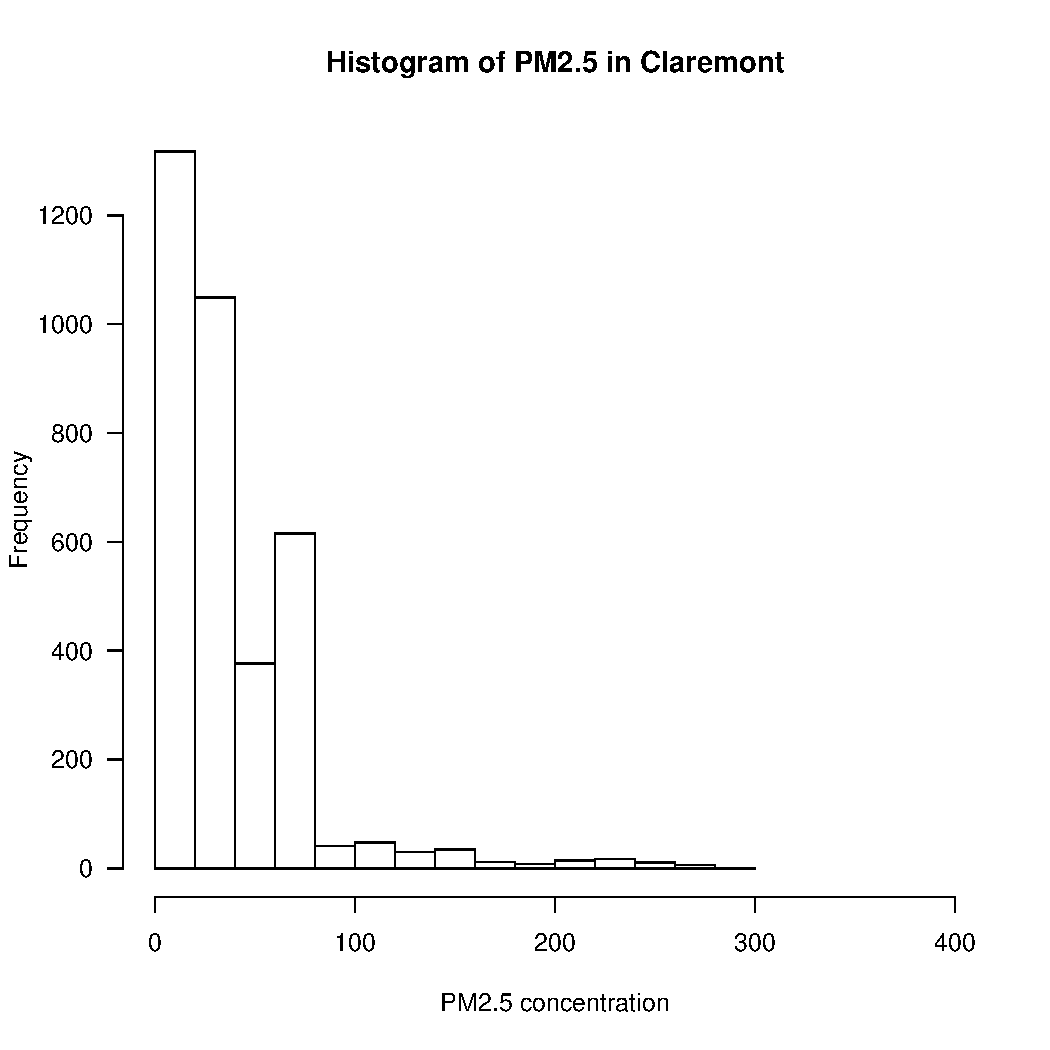
\includegraphics[width=\maxwidth]{figure/unnamed-chunk-3-1} 

\end{knitrout}

In my case, I have a very odd bimodal distribution and an long tail to boot. So, I am going plot on a time series to see if I can figure out what in the world is going on  (Figure~\ref{fig:draft}).

\begin{figure}
\begin{knitrout}
\definecolor{shadecolor}{rgb}{0.969, 0.969, 0.969}\color{fgcolor}\begin{kframe}
\begin{alltt}
\hlkwd{plot}\hlstd{(pm25_cf}\hlopt{~}\hlstd{DateTime,} \hlkwc{data}\hlstd{=cleandata,} \hlkwc{pch}\hlstd{=}\hlnum{20}\hlstd{,} \hlkwc{cex}\hlstd{=}\hlnum{.5}\hlstd{)}
\end{alltt}
\end{kframe}
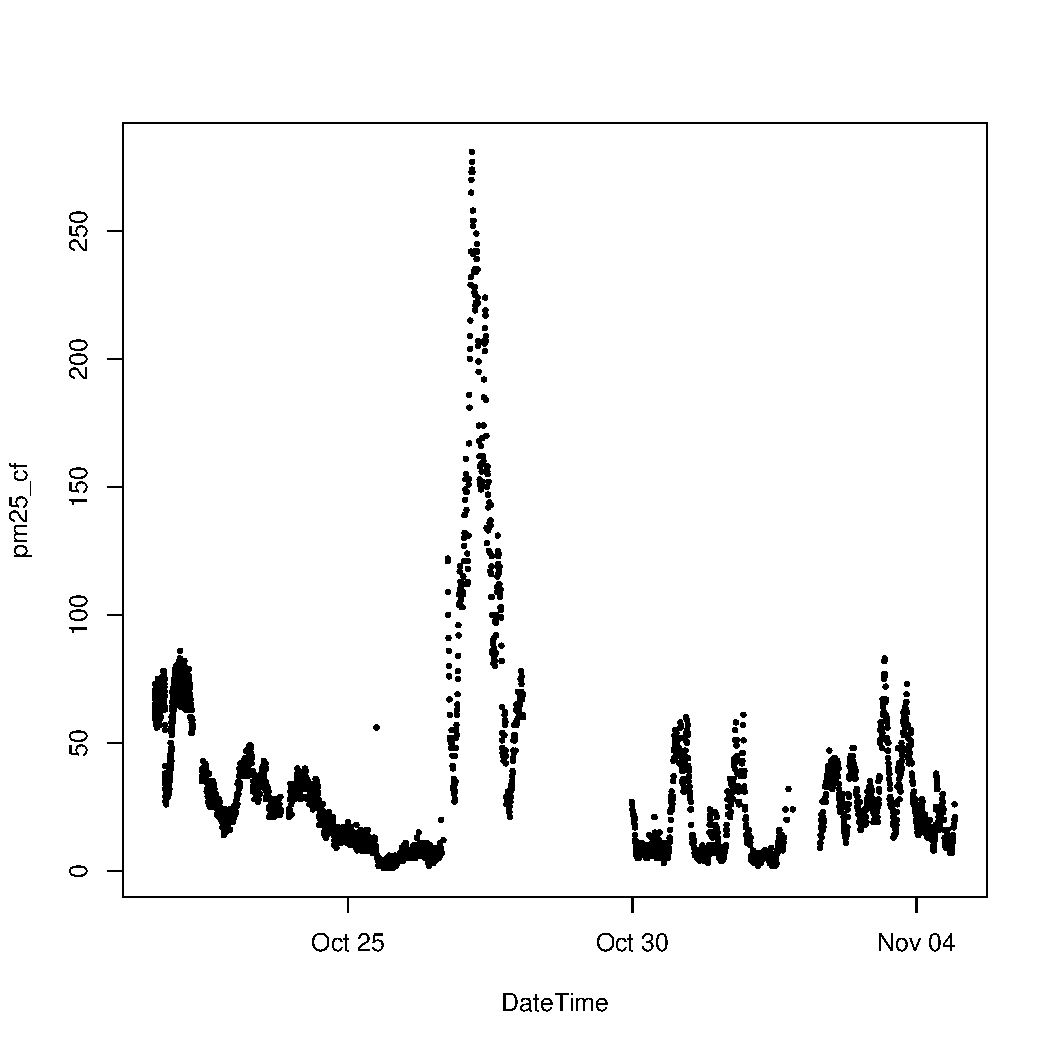
\includegraphics[width=\maxwidth]{figure/unnamed-chunk-4-1} 

\end{knitrout}
\caption{Draft Image -- needs work, but intersting patterns!}
\label{fig:draft}
\end{figure}
Except for some breaks in the data, we can certainly see a diurnal pattern, where the concentrations seem highest after midnight. 

Let's see if we can add times to the plot with some rectancles for ``night time''!  Furthermore, let's see how different size particles behave (Figure~\ref{fig:data}). 

\begin{figure}[h]
\begin{knitrout}
\definecolor{shadecolor}{rgb}{0.969, 0.969, 0.969}\color{fgcolor}
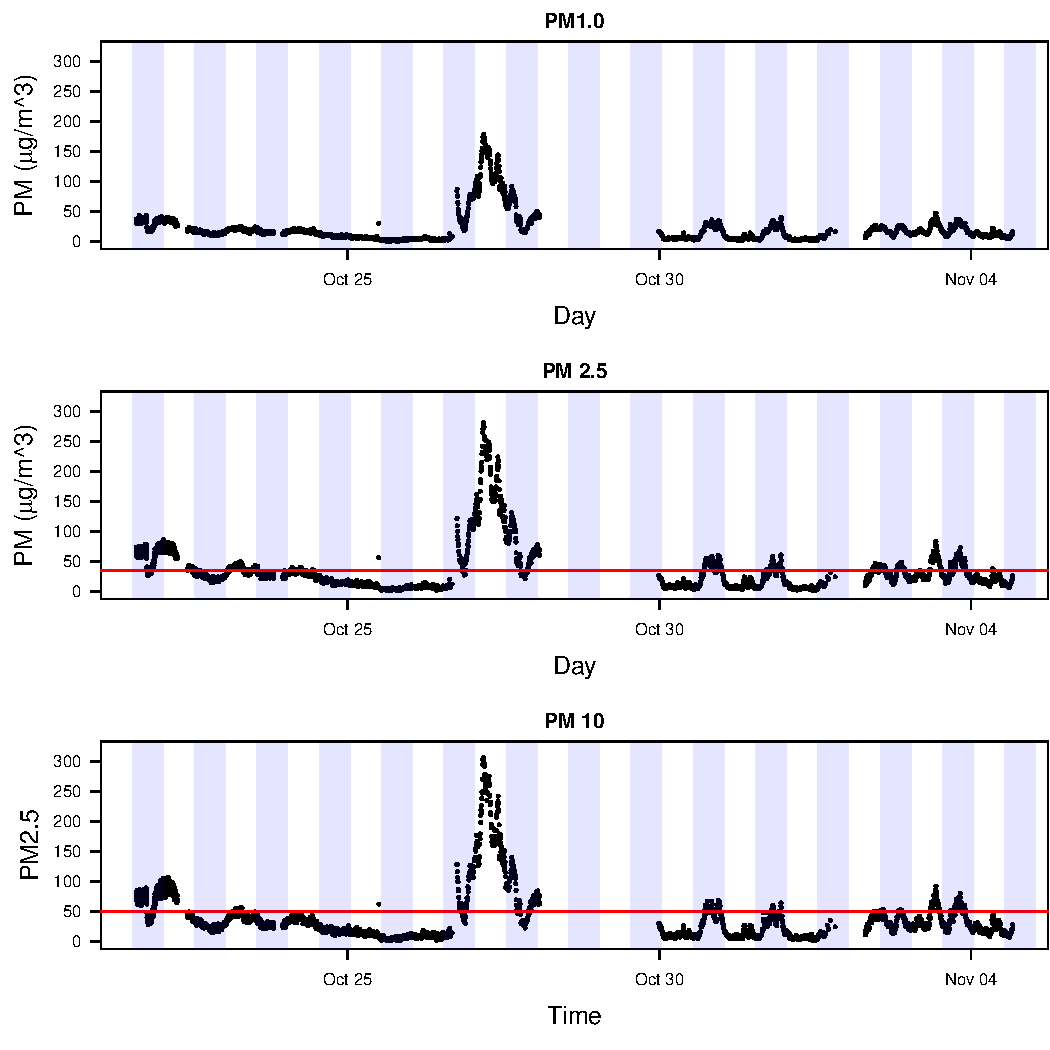
\includegraphics[width=\maxwidth]{figure/unnamed-chunk-5-1} 

\end{knitrout}
\caption{PM$_{1.0}$, PM$_{2.5}$ and PM$_{2.5}$ in Claremont California between Oct 21--Oct. 28, PM2.5 24 hour standard = 35, and PM10 24 hour standard = 50.}
\label{fig:data}
\end{figure}

Figure~\ref{} is not perfect. Here's a few issues:

\begin{itemize}
\item Dates and Days would be ideal
\item y-axis isn't quite correct
\item moving average might be nice. 
\item remove "dates" from top two figures because it's redundant.
\end{itemize}

For now, this is good enough -- and I'll keep working on this. Overall, Claremont's Air Quality was terrible on Wednesday night and Thursday morning. 

\section{Comparing Data to EPA Stations}

\subsection{Using previous collected data}

\begin{knitrout}
\definecolor{shadecolor}{rgb}{0.969, 0.969, 0.969}\color{fgcolor}\begin{kframe}
\begin{alltt}
\hlcom{# TBD}
\end{alltt}
\end{kframe}
\end{knitrout}

\subsection{Comparing $\mu$ to EPA Data}

The population mean (monthly average from the EPA data) is a parameter estimate. We can determine if the values you collected fall within the parameter estimate and it's 95\% confidence intervals. 

\begin{knitrout}
\definecolor{shadecolor}{rgb}{0.969, 0.969, 0.969}\color{fgcolor}\begin{kframe}
\begin{alltt}
\hlkwd{mean}\hlstd{(cleandata}\hlopt{$}\hlstd{pm1_cf)}
\end{alltt}
\begin{verbatim}
## [1] NA
\end{verbatim}
\end{kframe}
\end{knitrout}

Okay, now let's talk about signficant figures. The Pi only reports to the nearest whole value. Read about the rules in Wikipedia -- \url{https://en.wikipedia.org/wiki/Significant_figures}. In general, we should report to the whole number as well. However, some statiticians suggest that the mean and standard deviation can include one extra significant figure, allowing the reader to see the ``directionality'' of the mean toward the precision. However, for our purposes, I suggest we follow the standard rule and round to the nearest whole number and avoid implying additional precision.  

Finally, what happens if you get a missing value when using the function mean()?  Likely, this is due to missing values in the vector!  the mean function will not give you you an NA if NA is in the dataset. You can do a mean(DF, na.rm=T) to override the default\ldots

fyi: same as sd()

R wants users to be sure to understand the implications of missing data!  For example, what if we had missing data in cold temperatures -- then our mean would be biased!  When you decide to override the default, you want to be sure you are not introducing unknown biases\ldots

\section{More Intricate Analysis-- Based on Slack and Zooom Conversations :-)}

You could look to see if the there is a different during the time of the day or day of the week. You could move you sensor around in and outside your house and see if air quality is better / worse or the same\ldots.

We can help you with r code if you'd like to follow up with these additional questions. 

\subsection{Removing Missing Values}

Our Pi code seems to create missing data when the sensor doesn't respond in a timely fashion. 
\begin{knitrout}
\definecolor{shadecolor}{rgb}{0.969, 0.969, 0.969}\color{fgcolor}\begin{kframe}
\begin{alltt}
\hlkwd{summary}\hlstd{(cleandata)}
\end{alltt}
\begin{verbatim}
##     DateTime                       pm1_cf          pm25_cf      
##  Min.   :2020-10-21 14:32:25   Min.   :  0.00   Min.   :  1.00  
##  1st Qu.:2020-10-22 22:27:17   1st Qu.:  7.00   1st Qu.: 13.00  
##  Median :2020-10-26 09:43:06   Median : 17.00   Median : 29.00  
##  Mean   :2020-10-27 10:31:56   Mean   : 22.48   Mean   : 38.87  
##  3rd Qu.:2020-10-31 18:07:44   3rd Qu.: 32.00   3rd Qu.: 57.50  
##  Max.   :2020-11-04 16:09:13   Max.   :178.00   Max.   :281.00  
##  NA's   :2564                  NA's   :2574     NA's   :2574    
##     pm10_cf      
##  Min.   :  1.00  
##  1st Qu.: 14.00  
##  Median : 32.00  
##  Mean   : 43.56  
##  3rd Qu.: 64.00  
##  Max.   :306.00  
##  NA's   :2574
\end{verbatim}
\end{kframe}
\end{knitrout}
In my case, I have 2564 missing values! So, here's code to remove these missing values. Be sure you have not created a biased dataset by removing values that are systematically changing the accuracy!

\begin{knitrout}
\definecolor{shadecolor}{rgb}{0.969, 0.969, 0.969}\color{fgcolor}\begin{kframe}
\begin{alltt}
\hlstd{cleandata} \hlkwb{=} \hlkwd{na.omit}\hlstd{(cleandata)}
\hlkwd{summary}\hlstd{(cleandata)}
\end{alltt}
\begin{verbatim}
##     DateTime                       pm1_cf          pm25_cf      
##  Min.   :2020-10-21 14:32:25   Min.   :  0.00   Min.   :  1.00  
##  1st Qu.:2020-10-22 22:14:44   1st Qu.:  7.00   1st Qu.: 13.00  
##  Median :2020-10-26 09:15:25   Median : 17.00   Median : 29.00  
##  Mean   :2020-10-27 10:13:20   Mean   : 22.48   Mean   : 38.87  
##  3rd Qu.:2020-10-31 17:23:24   3rd Qu.: 32.00   3rd Qu.: 57.50  
##  Max.   :2020-11-04 16:09:13   Max.   :178.00   Max.   :281.00  
##     pm10_cf      
##  Min.   :  1.00  
##  1st Qu.: 14.00  
##  Median : 32.00  
##  Mean   : 43.56  
##  3rd Qu.: 64.00  
##  Max.   :306.00
\end{verbatim}
\end{kframe}
\end{knitrout}

\subsection{Subset for Dates or Times}

Let's say I want to compare day and night times. Let's say we compare 6:01 AM to 6 PM and 6:01 PM to 6:00 AM. 

I use a simple criteria to select data based on the hour -- using the libridate library.
\begin{knitrout}
\definecolor{shadecolor}{rgb}{0.969, 0.969, 0.969}\color{fgcolor}\begin{kframe}
\begin{alltt}
\hlkwd{library}\hlstd{(lubridate)}
\hlkwd{str}\hlstd{(cleandata)}
\end{alltt}
\begin{verbatim}
## 'data.frame':	3579 obs. of  4 variables:
##  $ DateTime: POSIXct, format: "2020-10-21 14:32:25" "2020-10-21 14:33:26" ...
##  $ pm1_cf  : num  32 36 33 35 31 34 35 34 33 35 ...
##  $ pm25_cf : num  64 73 65 68 62 68 70 67 61 63 ...
##  $ pm10_cf : num  75 77 73 80 73 82 78 79 75 68 ...
##  - attr(*, "na.action")= 'omit' Named int  79 93 104 176 180 212 246 325 339 377 ...
##   ..- attr(*, "names")= chr  "79" "93" "104" "176" ...
\end{verbatim}
\begin{alltt}
\hlstd{day} \hlkwb{=} \hlkwd{with}\hlstd{(cleandata,}
     \hlstd{cleandata[}\hlkwd{hour}\hlstd{(DateTime)}\hlopt{>} \hlnum{6} \hlopt{&}
               \hlkwd{hour}\hlstd{(DateTime)}\hlopt{<=} \hlnum{18}\hlstd{,])}

\hlstd{night} \hlkwb{=} \hlkwd{with}\hlstd{(cleandata,}
     \hlstd{cleandata[}\hlkwd{hour}\hlstd{(DateTime)}\hlopt{<=} \hlnum{6} \hlopt{&}
               \hlkwd{hour}\hlstd{(DateTime)}\hlopt{<} \hlnum{18}\hlstd{,])}
\end{alltt}
\end{kframe}
\end{knitrout}

Figure~\ref{fig:nightday} suggests that night time PM2.5 is higher, but let's check with a statistical test in section \ref{subsec:ttest}. 

\begin{figure}
\begin{knitrout}
\definecolor{shadecolor}{rgb}{0.969, 0.969, 0.969}\color{fgcolor}\begin{kframe}
\begin{alltt}
\hlkwd{boxplot}\hlstd{(day}\hlopt{$}\hlstd{pm25_cf, night}\hlopt{$}\hlstd{pm25_cf,} \hlkwc{names}\hlstd{=}\hlkwd{c}\hlstd{(}\hlstr{"Day"}\hlstd{,} \hlstr{"Night"}\hlstd{),} \hlkwc{las}\hlstd{=}\hlnum{1}\hlstd{)}
\end{alltt}
\end{kframe}
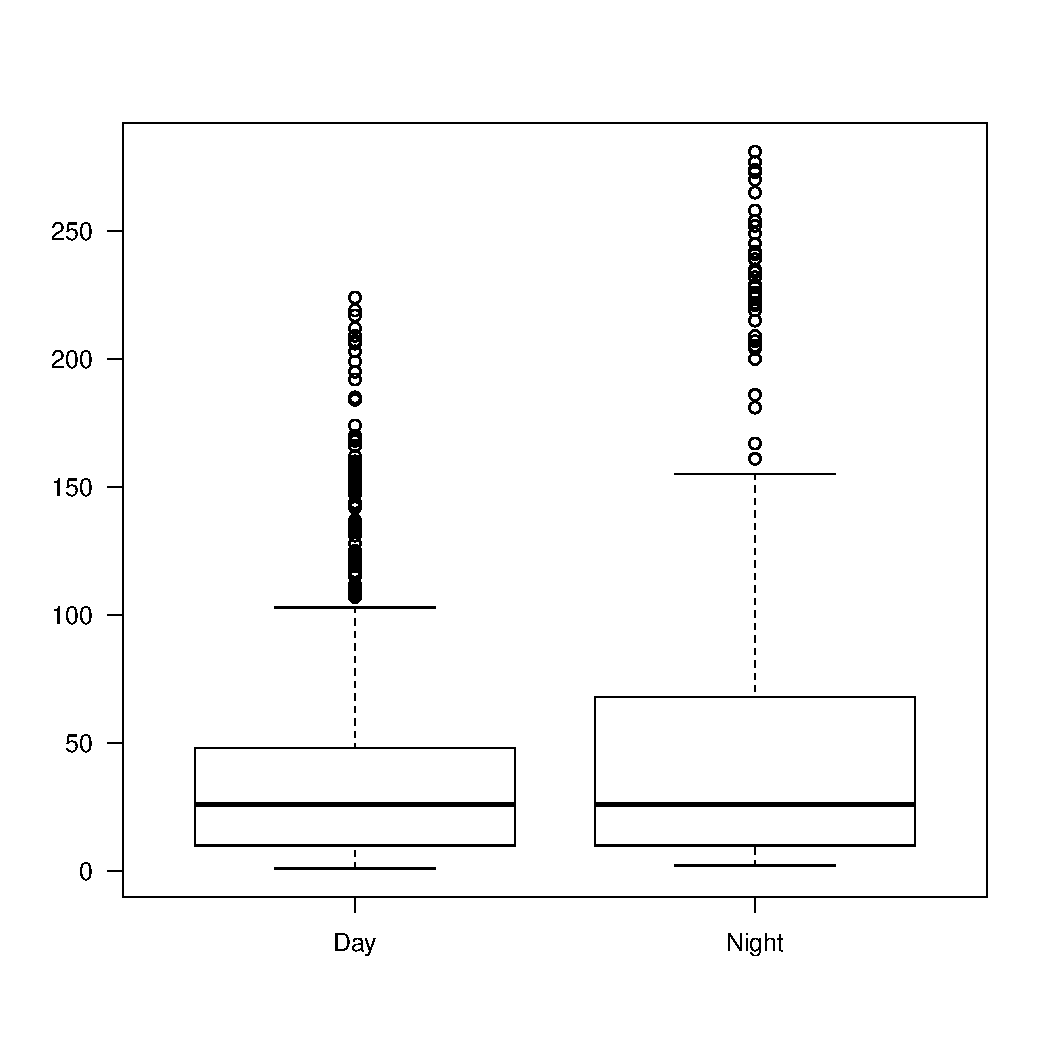
\includegraphics[width=\maxwidth]{figure/unnamed-chunk-11-1} 

\end{knitrout}
\caption{PM2.5 at day and night.}
\label{fig:nightday}
\end{figure}
Alternatively, let's select a period where a fire near Diamond Bar caused major air quality issue in Claremont.

\begin{knitrout}
\definecolor{shadecolor}{rgb}{0.969, 0.969, 0.969}\color{fgcolor}\begin{kframe}
\begin{alltt}
\hlkwd{str}\hlstd{(cleandata)}
\end{alltt}
\begin{verbatim}
## 'data.frame':	3579 obs. of  4 variables:
##  $ DateTime: POSIXct, format: "2020-10-21 14:32:25" "2020-10-21 14:33:26" ...
##  $ pm1_cf  : num  32 36 33 35 31 34 35 34 33 35 ...
##  $ pm25_cf : num  64 73 65 68 62 68 70 67 61 63 ...
##  $ pm10_cf : num  75 77 73 80 73 82 78 79 75 68 ...
##  - attr(*, "na.action")= 'omit' Named int  79 93 104 176 180 212 246 325 339 377 ...
##   ..- attr(*, "names")= chr  "79" "93" "104" "176" ...
\end{verbatim}
\begin{alltt}
\hlstd{fire} \hlkwb{=} \hlkwd{subset}\hlstd{(cleandata,}
  \hlkwc{subset}\hlstd{=}
    \hlstd{DateTime} \hlopt{>=} \hlkwd{as.Date}\hlstd{(}\hlstr{"2020-10-26 00:00:00"}\hlstd{)} \hlopt{&}
    \hlstd{DateTime} \hlopt{<=} \hlkwd{as.Date}\hlstd{(}\hlstr{"2020-10-28 00:00:00"}\hlstd{))}
\hlkwd{str}\hlstd{(fire)}
\end{alltt}
\begin{verbatim}
## 'data.frame':	498 obs. of  4 variables:
##  $ DateTime: POSIXct, format: "2020-10-26 00:00:28" "2020-10-26 00:05:50" ...
##  $ pm1_cf  : num  4 5 5 4 5 5 5 3 3 4 ...
##  $ pm25_cf : num  8 10 10 9 11 8 9 5 6 6 ...
##  $ pm10_cf : num  8 11 12 12 13 9 11 10 9 8 ...
\end{verbatim}
\end{kframe}
\end{knitrout}

\begin{knitrout}
\definecolor{shadecolor}{rgb}{0.969, 0.969, 0.969}\color{fgcolor}
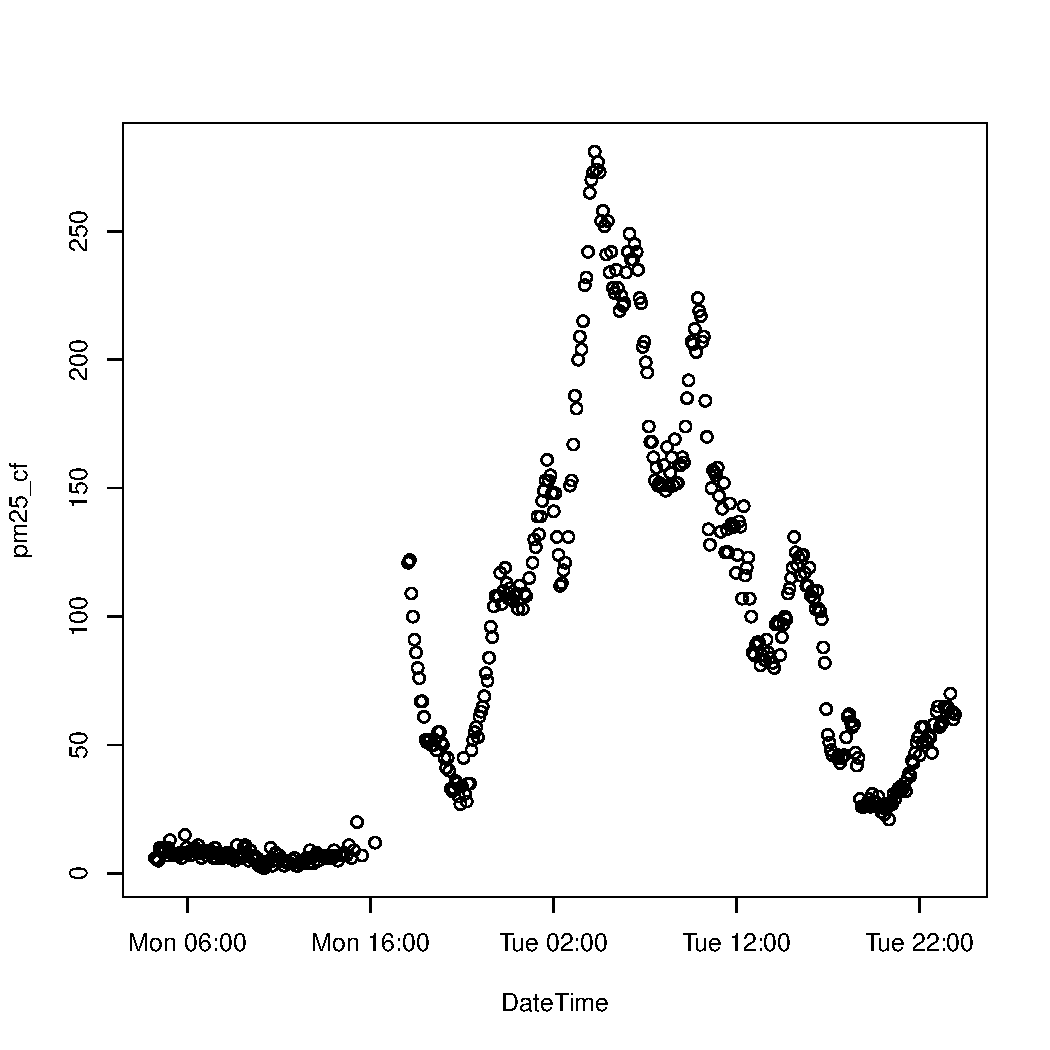
\includegraphics[width=\maxwidth]{figure/unnamed-chunk-13-1} 

\end{knitrout}

We might think of this as an event that might need to be analzyed in a different way!  

\subsection{Calculate 5/30 min averages}

How would you make a dataset of five minute intervals? We can use the dplyr library. 

Then we can use the function cut(), to create groups (based on time windows -- interestingly enough reponds to various word phrased for time, where ``5 min'' for five minute windows and ``30 min'' for 30 minute windows. 

\begin{knitrout}
\definecolor{shadecolor}{rgb}{0.969, 0.969, 0.969}\color{fgcolor}\begin{kframe}
\begin{alltt}
\hlkwd{str}\hlstd{(cleandata)}
\end{alltt}
\begin{verbatim}
## 'data.frame':	3579 obs. of  4 variables:
##  $ DateTime: POSIXct, format: "2020-10-21 14:32:25" "2020-10-21 14:33:26" ...
##  $ pm1_cf  : num  32 36 33 35 31 34 35 34 33 35 ...
##  $ pm25_cf : num  64 73 65 68 62 68 70 67 61 63 ...
##  $ pm10_cf : num  75 77 73 80 73 82 78 79 75 68 ...
##  - attr(*, "na.action")= 'omit' Named int  79 93 104 176 180 212 246 325 339 377 ...
##   ..- attr(*, "names")= chr  "79" "93" "104" "176" ...
\end{verbatim}
\begin{alltt}
\hlkwd{require}\hlstd{(dplyr)}
\end{alltt}


{\ttfamily\noindent\itshape\color{messagecolor}{\#\# Loading required package: dplyr}}

{\ttfamily\noindent\itshape\color{messagecolor}{\#\# \\\#\# Attaching package: 'dplyr'}}

{\ttfamily\noindent\itshape\color{messagecolor}{\#\# The following objects are masked from 'package:lubridate':\\\#\# \\\#\#\ \ \ \  intersect, setdiff, union}}

{\ttfamily\noindent\itshape\color{messagecolor}{\#\# The following objects are masked from 'package:stats':\\\#\# \\\#\#\ \ \ \  filter, lag}}

{\ttfamily\noindent\itshape\color{messagecolor}{\#\# The following objects are masked from 'package:base':\\\#\# \\\#\#\ \ \ \  intersect, setdiff, setequal, union}}\begin{alltt}
\hlstd{mean5min} \hlkwb{=} \hlstd{cleandata} \hlopt
  \hlkwd{group_by}\hlstd{(}\hlkwc{DateTime} \hlstd{=} \hlkwd{cut}\hlstd{(DateTime,} \hlkwc{breaks}\hlstd{=}\hlstr{"5 min"}\hlstd{))} \hlopt
  \hlkwd{summarize}\hlstd{(}\hlkwc{pm25_cf} \hlstd{=} \hlkwd{mean}\hlstd{(pm25_cf))}
\end{alltt}
\end{kframe}
\end{knitrout}


Or for 30 min means...
\begin{knitrout}
\definecolor{shadecolor}{rgb}{0.969, 0.969, 0.969}\color{fgcolor}\begin{kframe}
\begin{alltt}
\hlkwd{require}\hlstd{(dplyr)}
\hlstd{mean30min} \hlkwb{=} \hlstd{cleandata} \hlopt
  \hlkwd{group_by}\hlstd{(}\hlkwc{DateTime} \hlstd{=} \hlkwd{cut}\hlstd{(DateTime,} \hlkwc{breaks}\hlstd{=}\hlstr{"30 min"}\hlstd{))} \hlopt
  \hlkwd{summarize}\hlstd{(}\hlkwc{pm25_cf} \hlstd{=} \hlkwd{mean}\hlstd{(pm25_cf))}
\end{alltt}
\end{kframe}
\end{knitrout}

So, what did we create?  Let's look at the structure and head...

\begin{knitrout}
\definecolor{shadecolor}{rgb}{0.969, 0.969, 0.969}\color{fgcolor}\begin{kframe}
\begin{alltt}
\hlkwd{head}\hlstd{(mean30min)}
\end{alltt}
\begin{verbatim}
## # A tibble: 6 x 2
##   DateTime            pm25_cf
##   <fct>                 <dbl>
## 1 2020-10-21 14:32:00    65.0
## 2 2020-10-21 15:02:00    64.5
## 3 2020-10-21 15:32:00    64.9
## 4 2020-10-21 16:02:00    64.2
## 5 2020-10-21 16:32:00    65.3
## 6 2020-10-21 17:02:00    69.4
\end{verbatim}
\begin{alltt}
\hlkwd{str}\hlstd{(mean30min)}
\end{alltt}
\begin{verbatim}
## tibble [546 x 2] (S3: tbl_df/tbl/data.frame)
##  $ DateTime: Factor w/ 676 levels "2020-10-21 14:32:00",..: 1 2 3 4 5 6 7 8 9 10 ...
##  $ pm25_cf : num [1:546] 65 64.5 64.9 64.2 65.3 ...
\end{verbatim}
\end{kframe}
\end{knitrout}

This is a rather unique type of data set -- we are no looking at a "tibble", which is a particular type of data.frame that is structured as a table too. We also have lost our DateTime date formats, so this will not graph easily!  Ugh!!

\begin{knitrout}
\definecolor{shadecolor}{rgb}{0.969, 0.969, 0.969}\color{fgcolor}\begin{kframe}
\begin{alltt}
\hlkwd{plot}\hlstd{(pm25_cf} \hlopt{~} \hlstd{DateTime,} \hlkwc{data}\hlstd{=mean30min)}
\end{alltt}
\end{kframe}
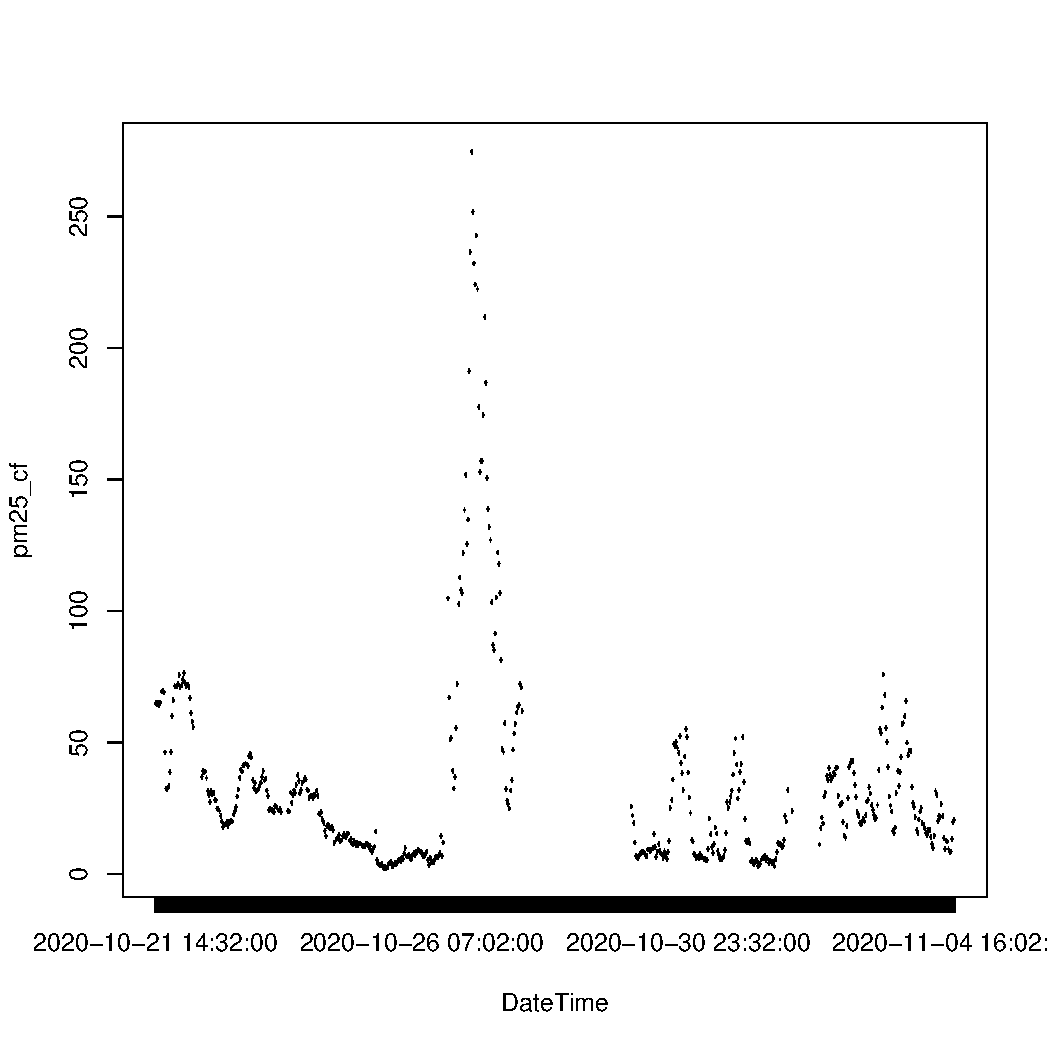
\includegraphics[width=\maxwidth]{figure/unnamed-chunk-17-1} 

\end{knitrout}
\noindent As a factor, we can't control the axis display very well -- and it looks like crap! The type of object doesn't seem to be bothering us much. So, let's march forward.

\begin{knitrout}
\definecolor{shadecolor}{rgb}{0.969, 0.969, 0.969}\color{fgcolor}\begin{kframe}
\begin{alltt}
\hlstd{mean30min}\hlopt{$}\hlstd{DateTime} \hlkwb{=} \hlkwd{as.POSIXct}\hlstd{(mean30min}\hlopt{$}\hlstd{DateTime,} \hlkwc{format}\hlstd{=}\hlstr{"%Y-%m-%d %H:%M:%S"}\hlstd{)}
\end{alltt}
\end{kframe}
\end{knitrout}

\begin{knitrout}
\definecolor{shadecolor}{rgb}{0.969, 0.969, 0.969}\color{fgcolor}\begin{kframe}
\begin{alltt}
\hlkwd{par}\hlstd{(}\hlkwc{mfrow}\hlstd{=}\hlkwd{c}\hlstd{(}\hlnum{2}\hlstd{,}\hlnum{1}\hlstd{),} \hlkwc{las}\hlstd{=}\hlnum{1}\hlstd{)}
\hlkwd{plot}\hlstd{(pm25_cf} \hlopt{~} \hlstd{DateTime,} \hlkwc{data}\hlstd{=mean30min,} \hlkwc{ty}\hlstd{=}\hlstr{"p"}\hlstd{,} \hlkwc{pch}\hlstd{=}\hlnum{20}\hlstd{,} \hlkwc{cex}\hlstd{=}\hlnum{.4}\hlstd{)}
\hlkwd{plot}\hlstd{(pm25_cf} \hlopt{~} \hlstd{DateTime,} \hlkwc{data}\hlstd{=mean30min,} \hlkwc{ty}\hlstd{=}\hlstr{"l"}\hlstd{)}
\end{alltt}
\end{kframe}
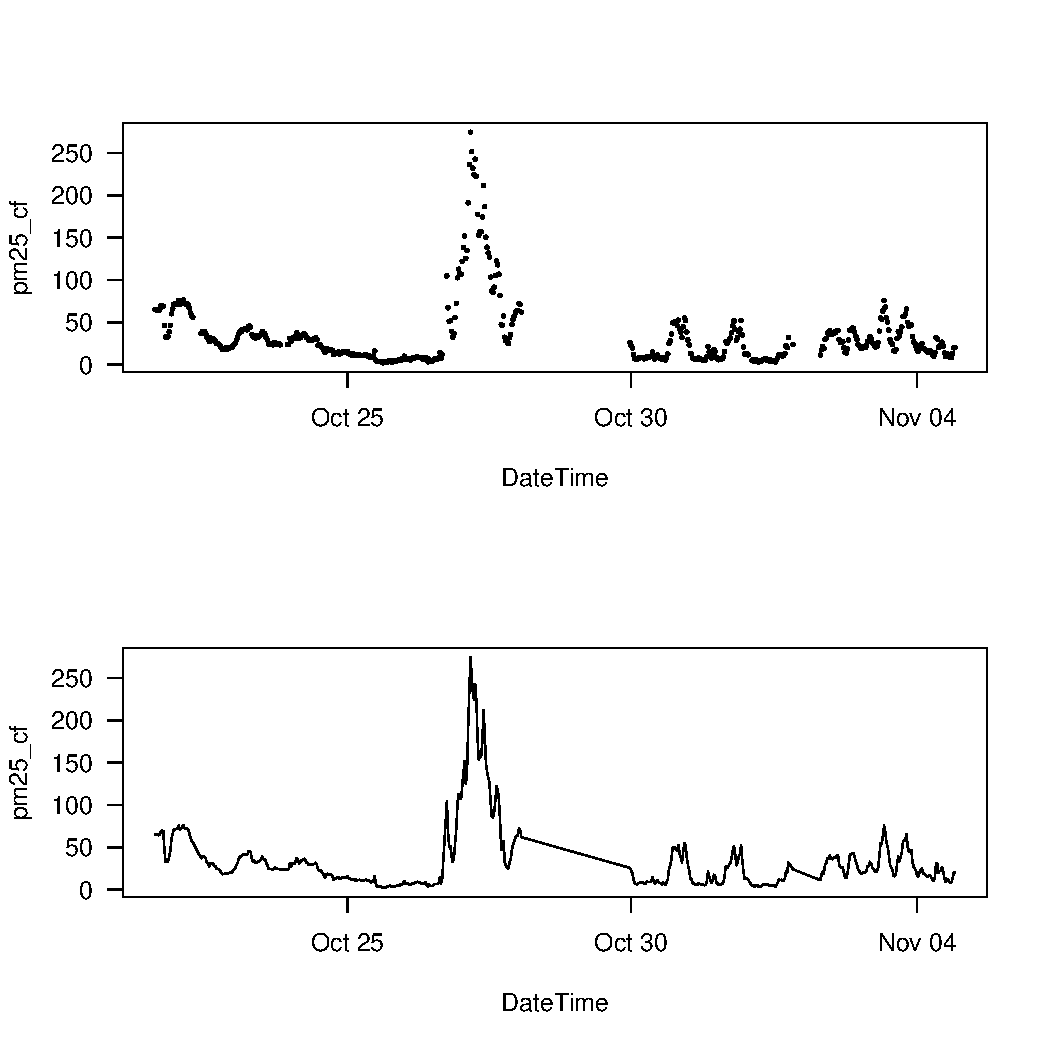
\includegraphics[width=\maxwidth]{figure/unnamed-chunk-19-1} 

\end{knitrout}

Note: when I make this a line graph (ty="l"), the missing data are a problem!  I will see how to fix that is someone asks, but I do like the display better than the point graphic.

let's see if we can limit the dates\ldots (Figure~\ref{fig:dualplot})

\begin{figure}
\begin{knitrout}
\definecolor{shadecolor}{rgb}{0.969, 0.969, 0.969}\color{fgcolor}\begin{kframe}
\begin{alltt}
\hlkwd{par}\hlstd{(}\hlkwc{mfrow}\hlstd{=}\hlkwd{c}\hlstd{(}\hlnum{1}\hlstd{,}\hlnum{2}\hlstd{),} \hlkwc{las}\hlstd{=}\hlnum{1}\hlstd{,} \hlkwc{pty}\hlstd{=}\hlstr{"s"}\hlstd{)}
\hlkwd{plot}\hlstd{(pm25_cf} \hlopt{~} \hlstd{DateTime,} \hlkwc{data}\hlstd{=mean30min,} \hlkwc{ty}\hlstd{=}\hlstr{"l"}\hlstd{,} \hlkwc{ylab}\hlstd{=}\hlstr{"Date"}\hlstd{)}
\hlkwd{plot}\hlstd{(pm25_cf} \hlopt{~} \hlstd{DateTime,} \hlkwc{data}\hlstd{=mean30min,} \hlkwc{ty}\hlstd{=}\hlstr{"p"}\hlstd{,}
  \hlkwc{pch}\hlstd{=}\hlnum{20}\hlstd{,} \hlkwc{cex}\hlstd{=}\hlnum{.4}\hlstd{,} \hlkwc{xlim}\hlstd{=}\hlkwd{c}\hlstd{(}\hlkwd{as.POSIXct}\hlstd{(}\hlstr{"2020-10-26 20:00:00"}\hlstd{),}
  \hlkwd{as.POSIXct}\hlstd{(}\hlstr{"2020-10-27 23:59:59"}\hlstd{)),} \hlkwc{ylab}\hlstd{=}\hlstr{"Conc"}\hlstd{,} \hlkwc{xaxt} \hlstd{=} \hlstr{"n"}\hlstd{,} \hlkwc{xlab}\hlstd{=}\hlstr{"Time"}\hlstd{)}

\hlstd{r} \hlkwb{<-} \hlkwd{as.POSIXct}\hlstd{(}\hlkwd{round}\hlstd{(}\hlkwd{range}\hlstd{(}\hlkwd{as.POSIXct}\hlstd{(}\hlstr{"2020-10-26 00:00:00"}\hlstd{),}
  \hlkwd{as.POSIXct}\hlstd{(}\hlstr{"2020-10-28 00:00:00"}\hlstd{)),} \hlstr{"hours"}\hlstd{))}

\hlkwd{axis.POSIXct}\hlstd{(}\hlnum{3}\hlstd{,} \hlkwc{at} \hlstd{=} \hlkwd{seq}\hlstd{(r[}\hlnum{1}\hlstd{], r[}\hlnum{2}\hlstd{],}
  \hlkwc{by} \hlstd{=} \hlstr{"day"}\hlstd{),} \hlkwc{format} \hlstd{=} \hlstr{"%D"}\hlstd{)}

\hlkwd{abline}\hlstd{(}\hlkwc{v}\hlstd{=}\hlkwd{as.POSIXct}\hlstd{(}\hlkwd{c}\hlstd{(}\hlstr{"2020-10-26 00:00:00"}\hlstd{,}
  \hlstr{"2020-10-27 00:00:00"}\hlstd{,} \hlstr{"2020-10-28 00:00:00"}\hlstd{)))}
\hlkwd{axis.POSIXct}\hlstd{(}\hlnum{1}\hlstd{,} \hlkwc{at} \hlstd{=} \hlkwd{seq}\hlstd{(r[}\hlnum{1}\hlstd{], r[}\hlnum{2}\hlstd{],}
  \hlkwc{by} \hlstd{=} \hlstr{"hour"}\hlstd{),} \hlkwc{format} \hlstd{=} \hlstr{"%H"}\hlstd{)}
\end{alltt}
\end{kframe}
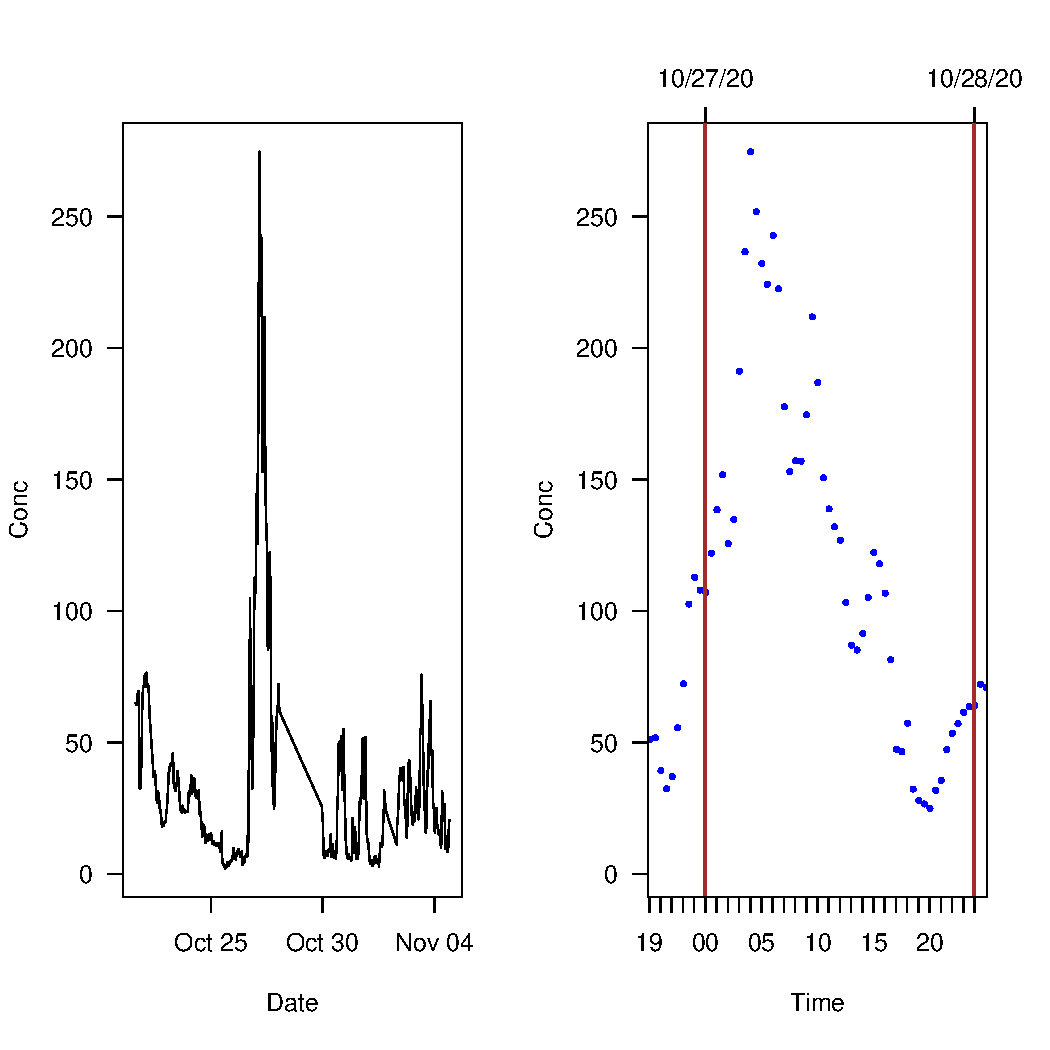
\includegraphics[width=\maxwidth]{figure/unnamed-chunk-20-1} 

\end{knitrout}
\caption{Focused Figure on PM change during a fire.}
\label{fig:dualplot}
\end{figure}

\clearpage
\subsection{Test test -- Comparing Two Populations}\label{subsec:ttest}

Now, let's formally test the null hypothesis that there is no difference between two populations of data -- night PM2.5 and day PM2.5
\begin{knitrout}
\definecolor{shadecolor}{rgb}{0.969, 0.969, 0.969}\color{fgcolor}\begin{kframe}
\begin{alltt}
\hlkwd{t.test}\hlstd{(day}\hlopt{$}\hlstd{pm25_cf, night}\hlopt{$}\hlstd{pm25_cf,} \hlkwc{pair}\hlstd{=}\hlnum{FALSE}\hlstd{)}
\end{alltt}
\begin{verbatim}
## 
## 	Welch Two Sample t-test
## 
## data:  day$pm25_cf and night$pm25_cf
## t = -4.4286, df = 1669, p-value = 1.01e-05
## alternative hypothesis: true difference in means is not equal to 0
## 95 percent confidence interval:
##  -11.234988  -4.337892
## sample estimates:
## mean of x mean of y 
##  35.68789  43.47433
\end{verbatim}
\end{kframe}
\end{knitrout}
\end{document}
